\documentclass[11pt,a4paper]{article}
\usepackage{float}
\usepackage{verbatim}
\usepackage{subfig}
\usepackage[T1]{fontenc}
\usepackage[utf8]{inputenc}
\usepackage{geometry}
\usepackage{enumitem}
%\geometry{verbose,lmargin=2cm,rmargin=2cm, bmargin=2cm, tmargin=2cm}
\usepackage{wrapfig}
\usepackage{tikz}
\usetikzlibrary{decorations.markings}
\usepackage{calc}
\usepackage{wrapfig}
\usepackage{graphicx}
\usepackage{amssymb}
\usepackage{amsmath}
\usepackage{esint}
\usepackage{multicol}
\usepackage{hyperref}
\usepackage{listings}
\hypersetup{
    colorlinks=true,
    linkcolor=blue,
    filecolor=magenta,
    urlcolor=cyan,
}
\usepackage{listings}
\lstset{ %
  backgroundcolor=\color{white},   % choose the background color; you must add \usepackage{color} or \usepackage{xcolor}; should come as last argument
  basicstyle=\footnotesize,        % the size of the fonts that are used for the code
  breakatwhitespace=false,         % sets if automatic breaks should only happen at whitespace
  breaklines=true,                 % sets automatic line breaking
  captionpos=t,                    % sets the caption-position to bottom
  commentstyle=\color{teal},    % comment style
  deletekeywords={...},            % if you want to delete keywords from the given language
  escapeinside={\%*}{*)},          % if you want to add LaTeX within your code
  extendedchars=true,              % lets you use non-ASCII characters; for 8-bits encodings only, does not work with UTF-8
  frame=single,                    % adds a frame around the code
  keepspaces=true,                 % keeps spaces in text, useful for keeping indentation of code (possibly needs columns=flexible)
  keywordstyle=\color{blue},       % keyword style
 % language=Python,                 % the language of the code
  morekeywords={*,...},           % if you want to add more keywords to the set
  numbers=left,                    % where to put the line-numbers; possible values are (none, left, right)
  numbersep=5pt,                   % how far the line-numbers are from the code
  numberstyle=\tiny\color{black}, % the style that is used for the line-numbers
  rulecolor=\color{black},         % if not set, the frame-color may be changed on line-breaks within not-black text (e.g. comments (green here))
  showspaces=false,                % show spaces everywhere adding particular underscores; it overrides 'showstringspaces'
  showstringspaces=false,          % underline spaces within strings only
  showtabs=false,                  % show tabs within strings adding particular underscores
  stepnumber=1,                    % the step between two line-numbers. If it's 1, each line will be numbered
  tabsize=2,                       % sets default tabsize to 2 spaces
  title=\lstname                   % show the filename of files included with \lstinputlisting; also try caption instead of title
}
\begin{document}



%\preprint{APS/123-QED}

\title{FYS2150 \\ Lab Report: Drag}% Force line breaks with \\

\author{Nicholas Karlsen}
% \email{nichoka@student.matnat.uio.no}

\date{\today}% It is always \today, today,
             %  but any date may be explicitly specified

\maketitle

\begin{abstract}
  A study on the flow of an assortment of spheres in a fluid and the use of image processing to determine the terminal velocity.
\end{abstract}

%\tableofcontents

\begin{multicols*}{2}
\section{\label{sect:intro}Introduction}
  This report contains the description and analysis of data collected in the lab 21.03.2018 concerning the flow of several spherical objects in a large range of different sizes and densities. The balls were immersed in fluid, dropped and filmed. Post-lab, the raw footage was then processed using a Python script in order to quantify the motion of the spheres. This 

\section{\label{sect:theory}Theory}

\section{\label{section:experimental}Experimental Procedure} 
  \subsection{Video capture}
    
    \begin{figure}[H]
      \center
      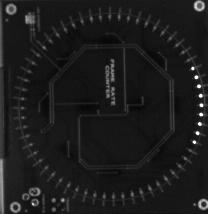
\includegraphics[width=7cm]{scripts/figs/sync_fps.png}
      \caption{Signal used to determine the FPS of the camera}
      \label{fig:FpsSignal}
    \end{figure}
  

    In order to capture the motion of the balls, a USB video camera was connected to a computer running uEye cockpit \cite{website:ueye}, which we used to change the settings of the camera and make recordings.
    In order to ensure that the footage was suitable to be analyzed using the image processing techniques described earlier several of the parameters in uEye cockpit had to be manually adjusted. 

    First, the error of the stated FPS of the camera had to be determined. This was done by connecting a series of circular LEDs (see Fig. \ref{fig:FpsSignal}) to a signal generator. The light emitted would "circle" at a rate which could be changed using the signal generator. By adjusting the signal such that the emitted light would seem stationary when observed through the video feed in uEye cockpit, the FPS of the camera determined to be 
    

  \begin{figure}[h]
    \center
    \subfloat[][Large tube]{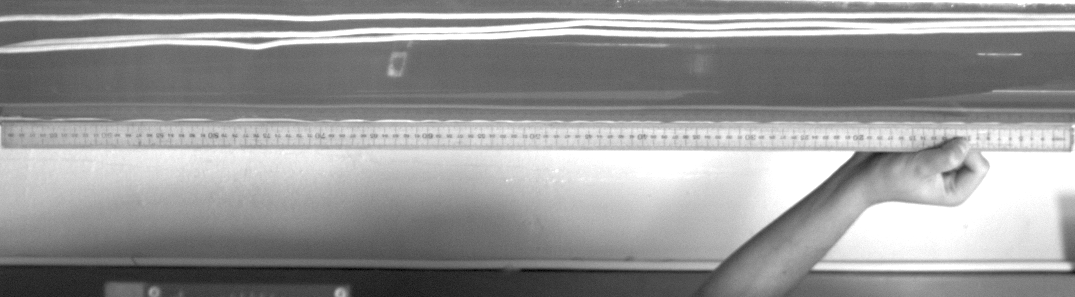
\includegraphics[width=8cm, angle=90]{scripts/figs/bilde_scale1.png}\label{<figure1>}}
    \subfloat[][Small tube]{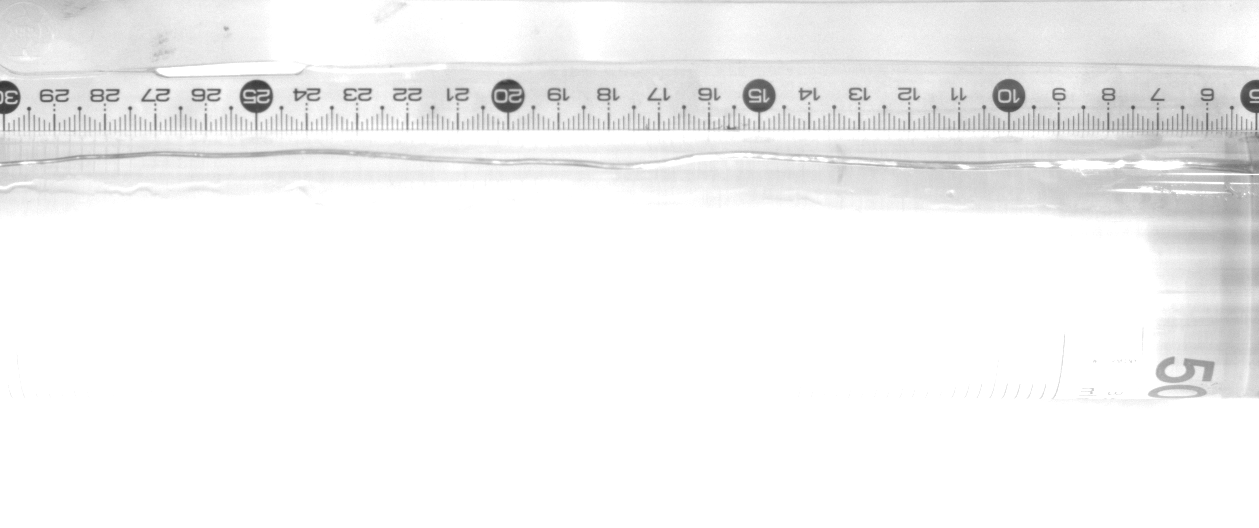
\includegraphics[width=8cm, angle=90]{scripts/figs/bilde_scale2.png}\label{<figure1>}}

    \caption{Cropped images used to find pixel to meter ratio for both of the tubes. (Scaled down in this document)}
    \label{fig:scale1}
  \end{figure}

  \begin{figure}[H]
    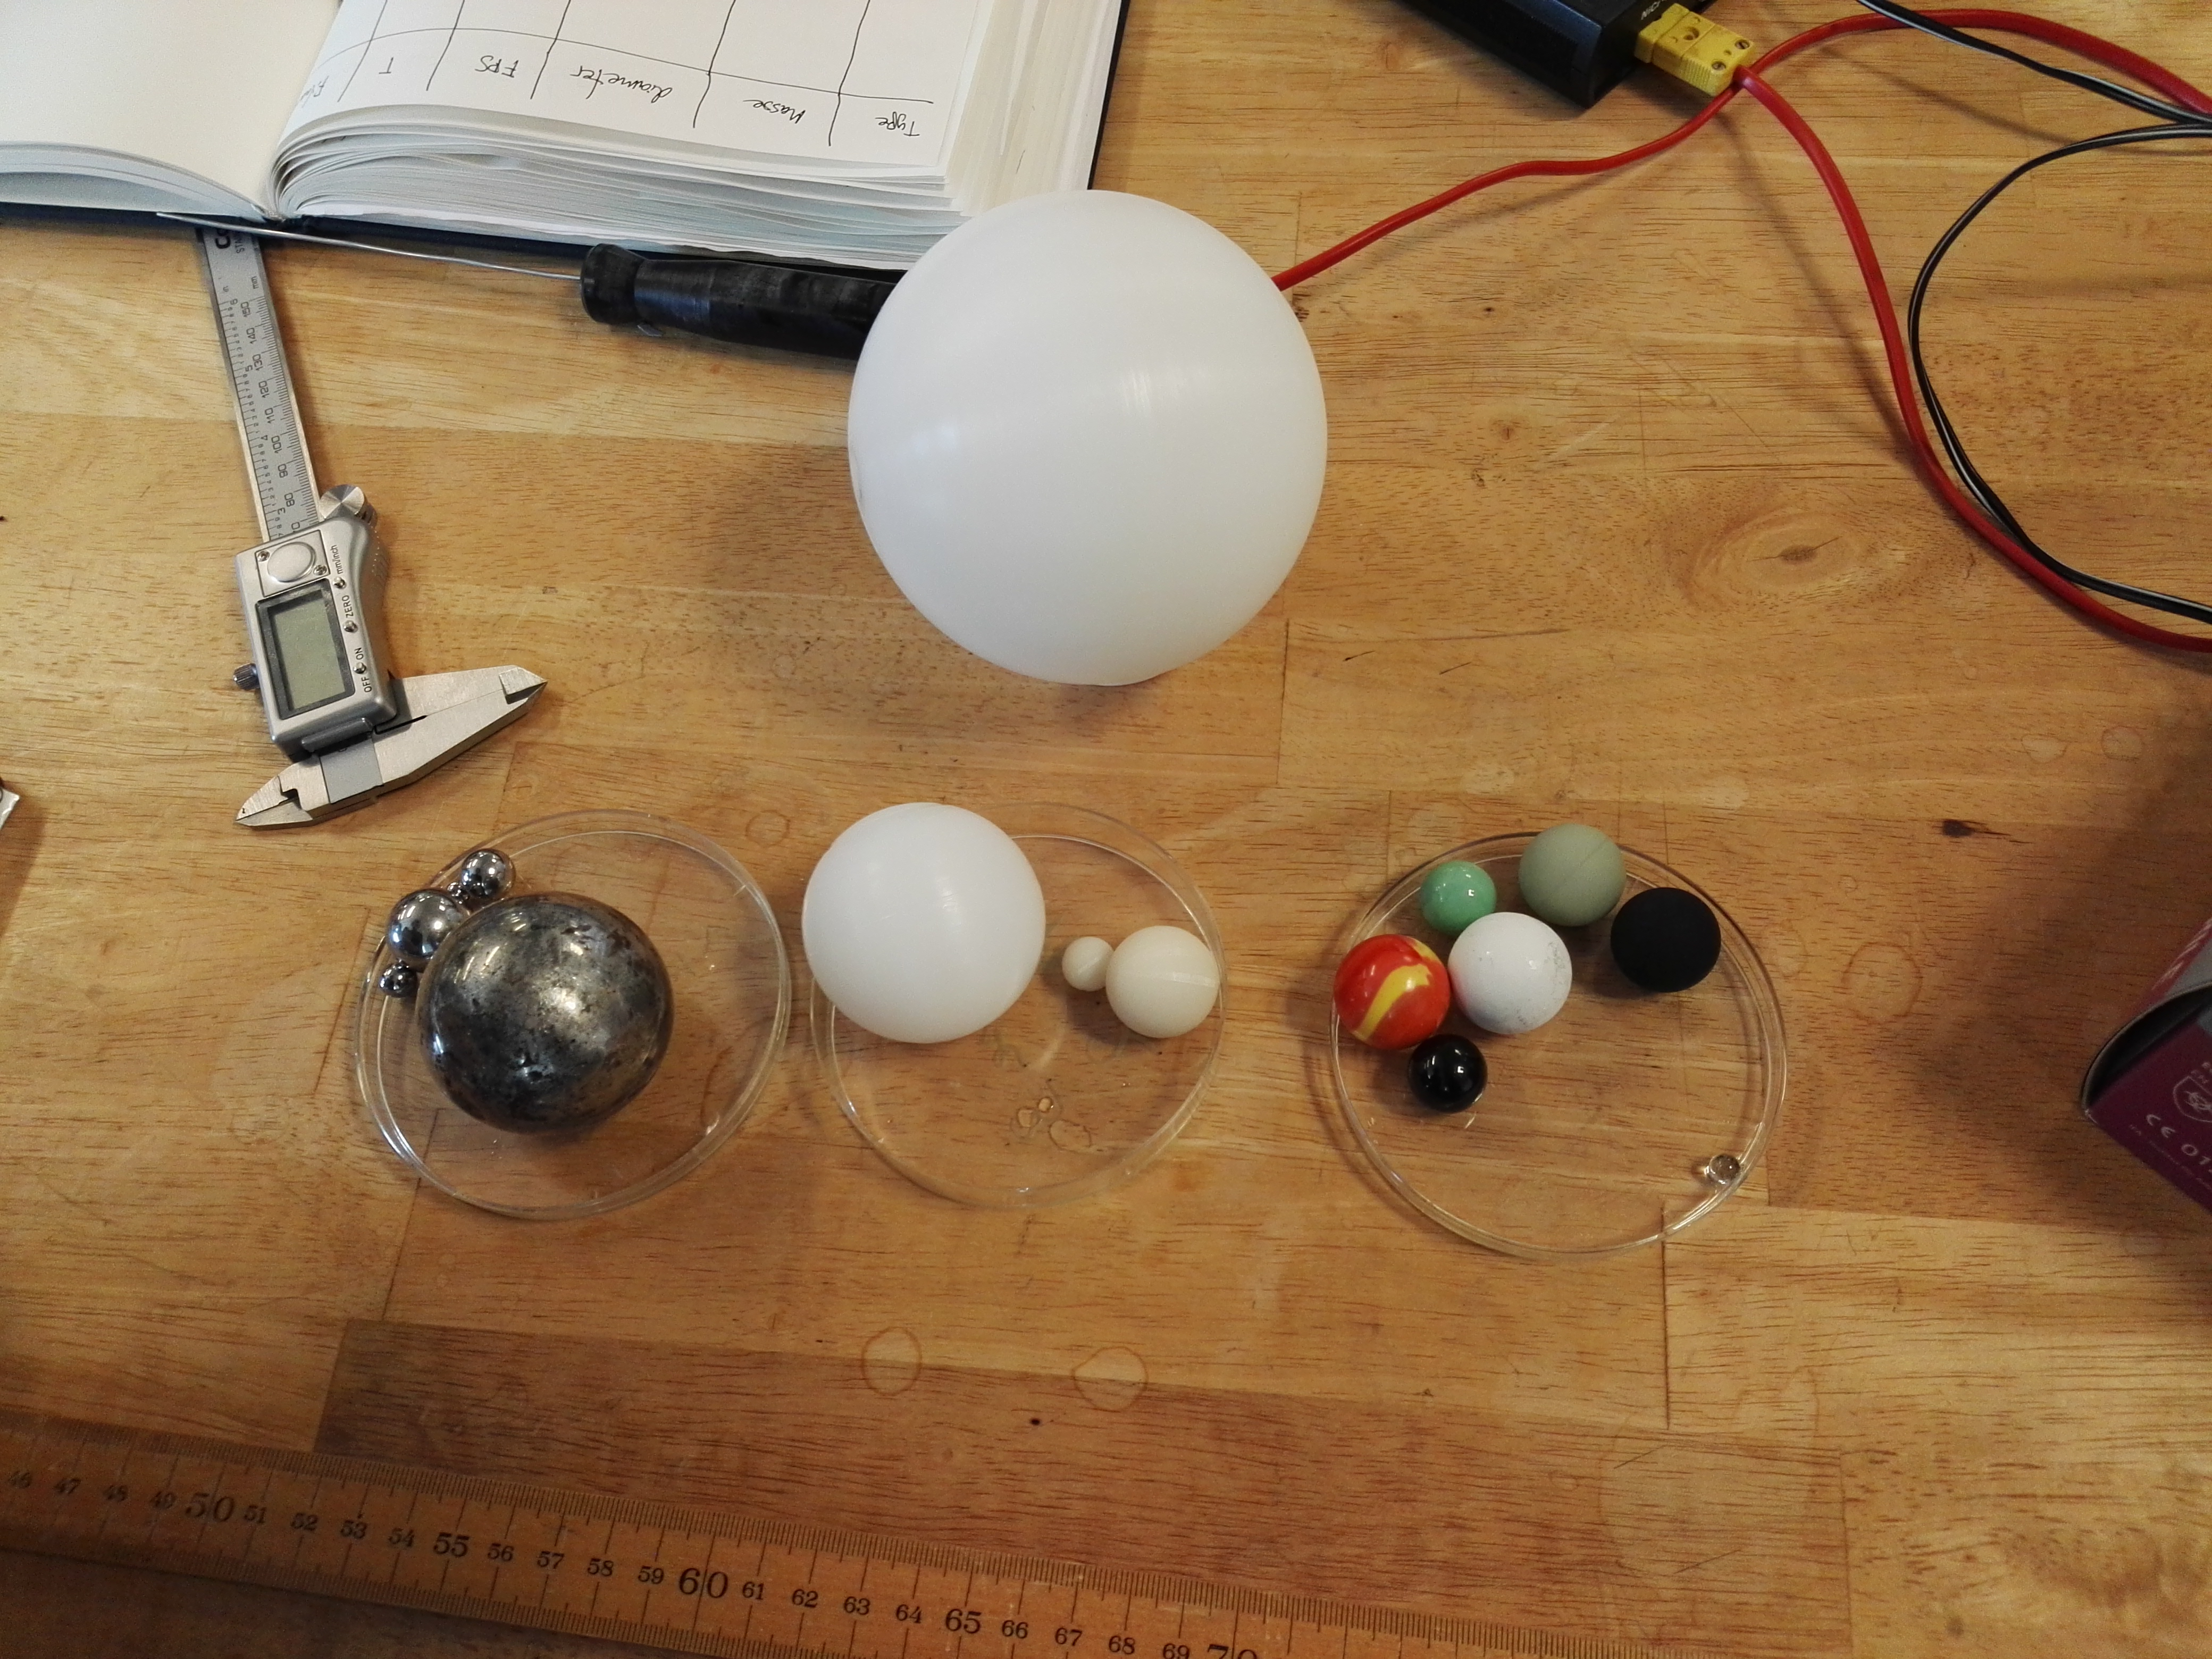
\includegraphics[width=7cm]{scripts/figs/IMG_20180321_131204.jpg}
    \caption{Most of the balls used in the experiment, excluding the ones labeled small 1 and 2.}
  \end{figure}


\section{\label{sect:results}Results}
\end{multicols*}

  \begin{table}[H]
    \center
    \begin{tabular}{ r | l  l  r  r  r }
      
      Type       & Mass [g] & Diameter [mm]   & FPS    & T [$^\circ$C]   & Filename \\ 
      \hline
      Metal       & 502.76  & 48.98          & 100    & 22.7   & A1.avi  \\ 
      Metal       & 28.13   & 19.02          & 100    & 22.8   & A2.avi  \\  
      Metal       & 6.99    & 11.97          & 100    & 22.6   & A3.avi  \\ 
      Metal       & 2.08    & 7.99           & 100    & 22.6   & A4.avi  \\ 
      Metal       & 0.68    & 5.48           & 100    & 22.5   & A5.avi  \\ 
      Metal       & 0.10    & 2.98           & 100    & 22.6   & A6.avi  \\ 
      \\
      Plastic     & 488.41  & 99.4           & 100    & 22.5   & B1.avi  \\ 
      Plastic     & 61.56   & 50.02          & 100    & 22.5   & B2.avi  \\ 
      Plastic     & 7.12    & 23.89          & 100    & 22.6   & B3.avi  \\ 
      Plastic     & 0.87    & 12.06          & 100    & 22.6   & B4.avi  \\ 
      \\
      White       & 29.74   & 25.24          & 100    & 22.6   & C1.avi  \\ 
      BigB lack   & 31.42   & 21.08          & 100    & 22.5   & C4.avi  \\ 
      Small Black & 5.67    & 16.45          & 100    & 22.5   & C5.avi  \\ 
      Big Green   & 31.60   & 21.86          & 100    & 22.4   & C3.avi  \\ 
      Small Green & 5.60    & 16.38          & 100    & 22.3   & C6.avi  \\ 
      Big Red     & 18.44   & 24.01          & 100    & 22.3   & C2.avi  \\ 
      Glass       & 0.27    & 5.81           & 100    & 22.3   & C7.avi  \\ 
      \\
      Small 2     & 12.0E-3 & 1.59           & 100    & 23.7   & D2.avi  \\    
      Small 1     & 4.1E-3  & 1.0            & 100    & 23.7   & D1.avi  \\ 
    \end{tabular}
    \caption{Spheres}
  \end{table}

\begin{multicols*}{2}

\section{\label{sect:discuss}Discussion}
\section{\label{sect:conclusion}Conclusion}

\bibliographystyle{plain}
\bibliography{references} 

\end{multicols*}

%%%%%%%%%%%%%%%%%%%%%%%%
%%% END OF MAIN BODY %%%
%%%%%%%%%%%%%%%%%%%%%%%%

\appendix*
\section{Code}
Following

\lstinputlisting[language=python]{scripts/lesVideo_conv.py}
\lstinputlisting{scripts/data/labdata.dat}

\end{document}